\begin{frame}{今回の形状作成の概要}
  %
   \begin{columns}[t]
    \begin{column}{0.6\textwidth}
      <今回の形状作成の概要>
      \begin{itemize}
        \item[(1)]<1-> ます、側面の板を作って
	\item[(2)]<2-> 回転押し出し
	\item[(3)]<3-> レンガ状に切断
	\item[(4)]<4-> 回転中心軸に面積0の縮退面発生 \\
		       条件に違反のため6面体メッシュが \\
		       切れない
	\item[(5)]<5-> 左下の正常なブロックを回転コピー
      \end{itemize}
    \end{column}
    \begin{column}{0.4\textwidth}
      \vspace{-7mm}
      \begin{figure}[htbp]
        \begin{center}
	  \begin{overlayarea}{7cm}{15cm}
	    \only<1>{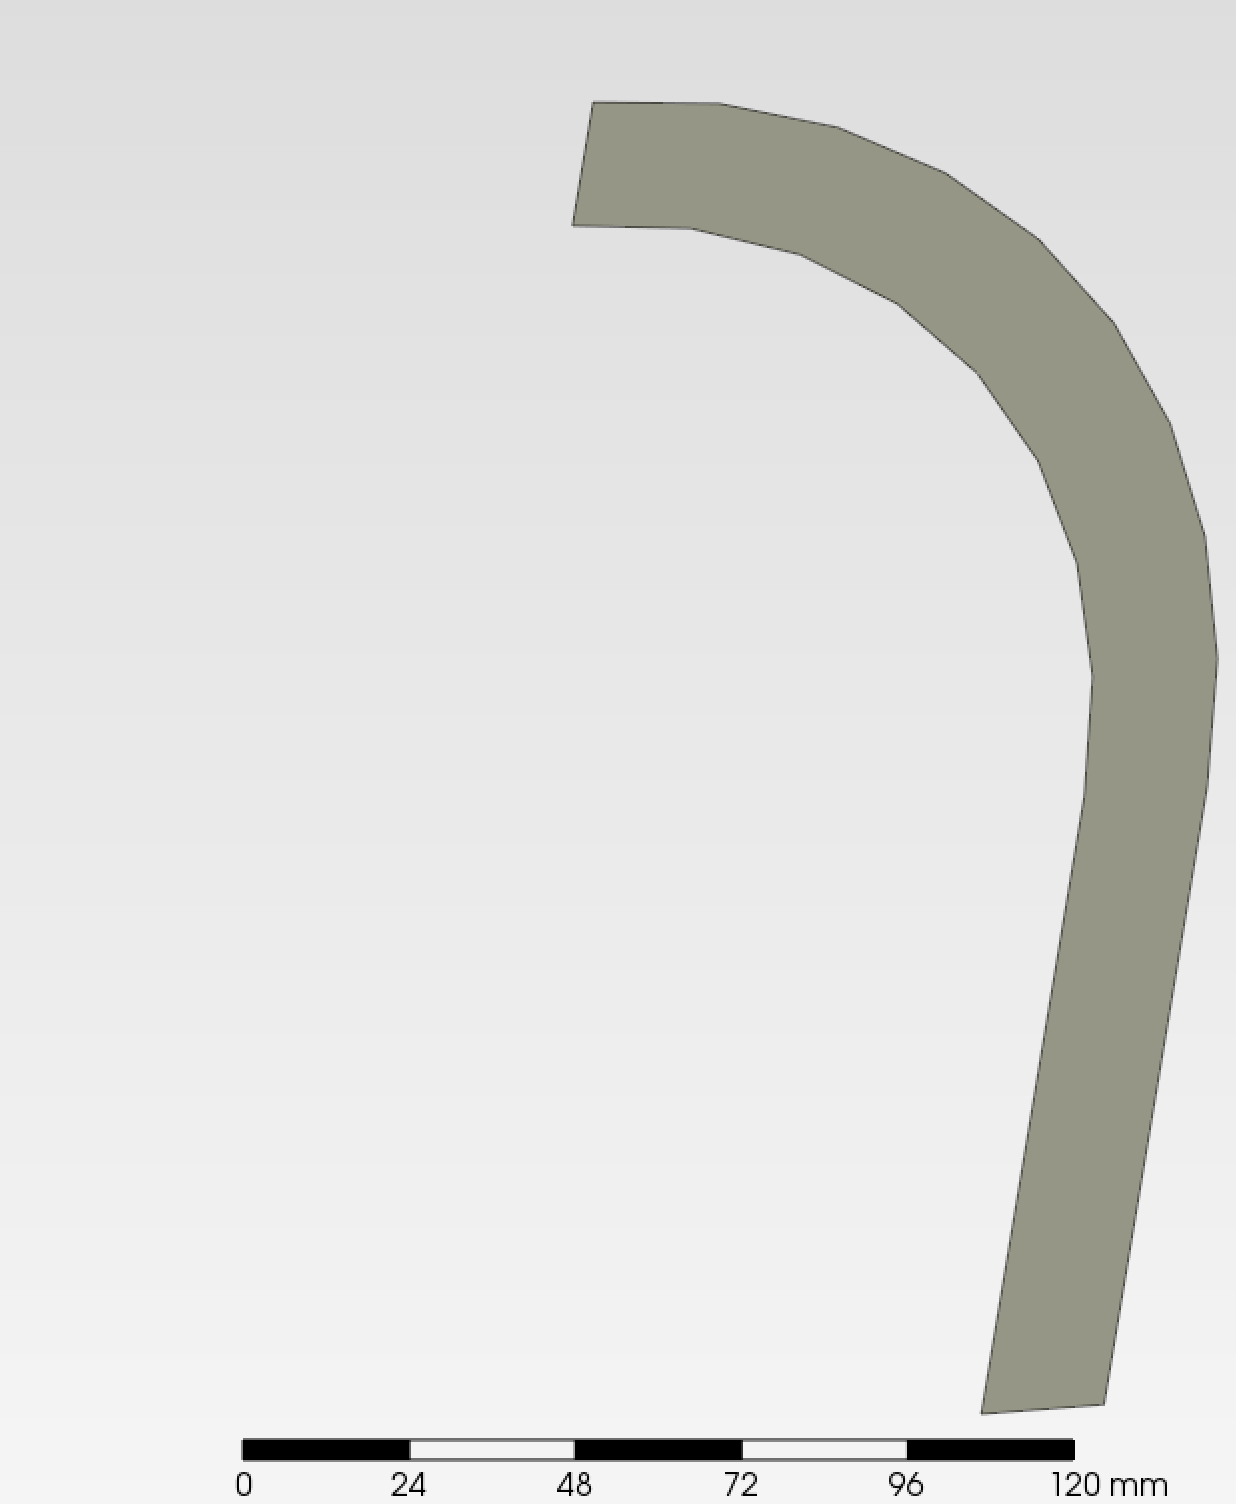
\includegraphics[keepaspectratio,scale=0.35]{images/sc1.png}}
	    \only<2>{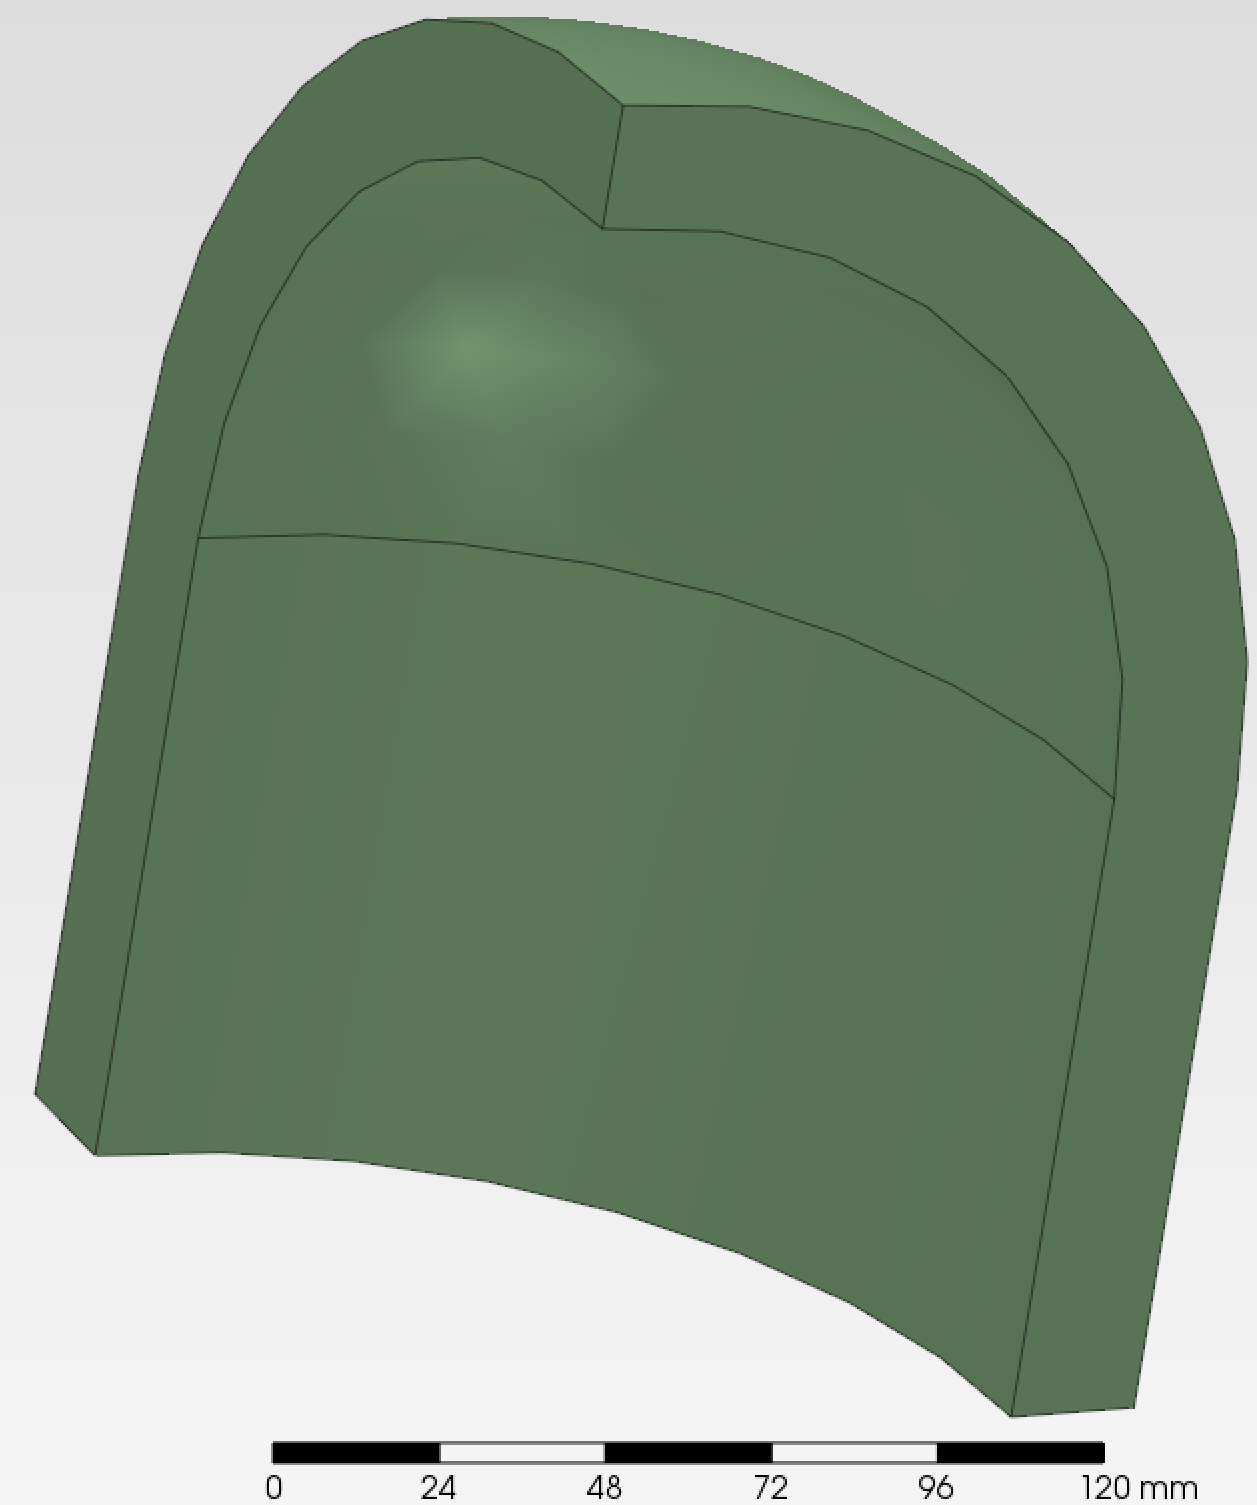
\includegraphics[keepaspectratio,scale=0.35]{images/sc2.png}}
	    \only<3->{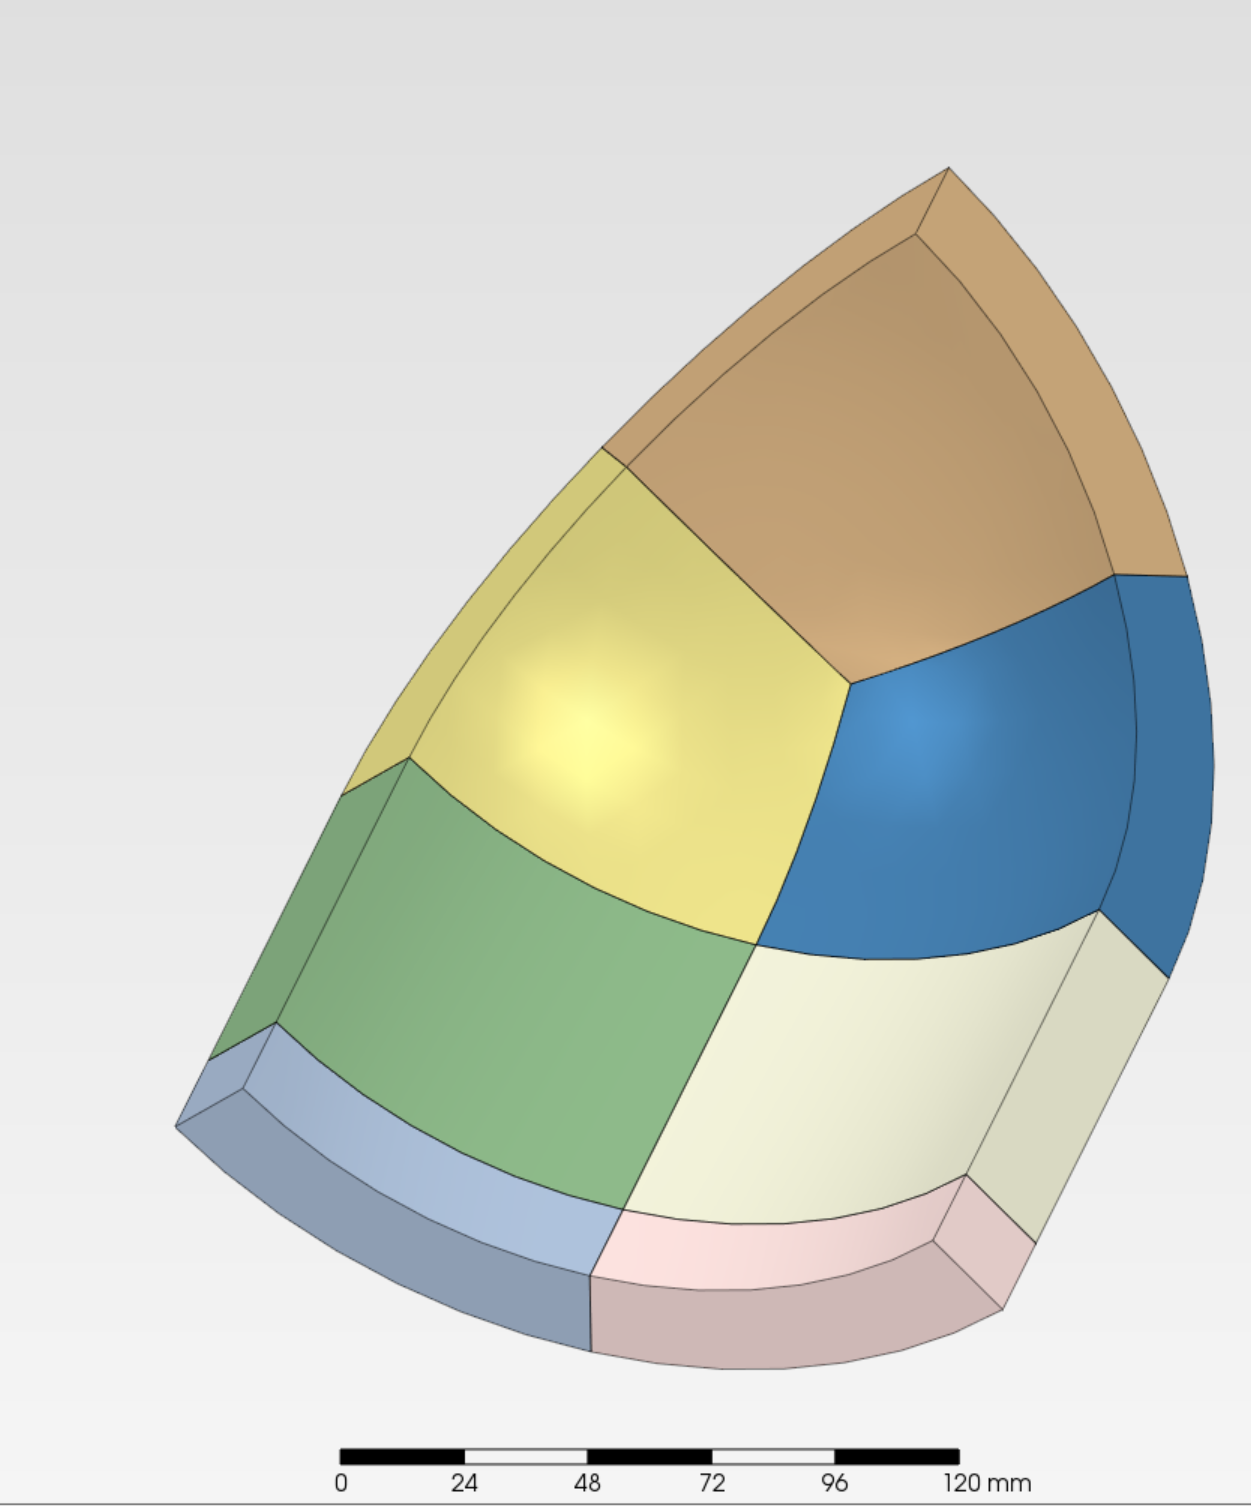
\includegraphics[keepaspectratio,scale=0.35]{images/sc3.png}}
            \caption{形状作成法の概要}
	  \end{overlayarea}
        \end{center}
      \end{figure}
    \end{column}
  \end{columns}
  \only<4>{
    \begin{textblock*}{30pt}(255pt,40pt)
      \begin{tikzpicture}
         \node[rectangle,fill=cud_yellow,text width=0.5cm,text centered,rounded corners,minimum height=0.5cm](s) at (1cm,1cm) { \scriptsize 面積0の縮退面};
         \draw[->, draw=cud_red, line width=1pt] (40pt,50pt) -- (133pt,70pt);
         \draw[draw=cud_red, line width=2pt] (133pt,66pt) -- (138pt,76pt);
      \end{tikzpicture}
    \end{textblock*}
  }
  \only<5>{
    \begin{textblock*}{30pt}(255pt,40pt)
      \begin{tikzpicture}
         \node[rectangle,fill=cud_yellow,text width=0.5cm,text centered,rounded corners,minimum height=0.5cm](s) at (1cm,1cm) { \scriptsize 回転コピ|};
         \draw[->, draw=cud_red, line width=1pt] (40pt,30pt) -- (95pt,0pt);
         \draw[->, draw=cud_red, line width=2pt] (103pt,-20pt) to [bend left=90]  (128pt,20pt);
      \end{tikzpicture}
    \end{textblock*}
  }
\end{frame}
